% !TEX root = ./report.tex

\clearpage
\section{The Inliner}
\label{sec:scheme}

Our inliner utilizes Jive's RVSDG IR functionality to perform the inlining on
the inputted assembly code program. As such, the inliner is both compiled into
Jive, and utilizes functionalities offered by Jive. This section details the
actions performed by the inliner, and the reasoning behind these. First, we give
an overview of the actions performed by the inliner, before we go more into
depth on the reasoning behind them.

Following is the algorithm representing the steps executed by the inliner:

\begin{enumerate}
	\item For all recursive environments ($\phi$-regions):

	\begin{enumerate}
		\item Use the approach described in
Section~\ref{sub:scheme:inlining_recur_apply_nodes} to fill a list of
\textit{loop breakers}. These functions ($\lambda$-nodes) are \textit{not} to be
inlined.
		\label{MakeLoopBreakerListItem}
	\end{enumerate}

	\item Scan through the RVSDG, finding all call sites (\applyNode s). Exclude
all function calls to loop breakers, calls invoking functions which are not
statically known, or external functions.
	\label{ScanForApplyNodesItem}

	\item Make a list of the \applyNode s found in
Step~\ref{ScanForApplyNodesItem}, and order the list according to the heuristics
discussed in Section~\ref{sub:scheme:ordering_apply_nodes}. The order of
\applyNode s inlined can affect the total amount of \applyNode s inlined, even
when all of the \applyNode s are evaluated with the same heuristic.
\label{OrderApplyNodesFoundItem}

	\item Look at each \applyNode~in turn from the list made in
Step~\ref{OrderApplyNodesFoundItem} and decide whether or not to inline it
according to the heuristic discussed in
Section~\ref{sub:scheme:inlining_apply_nodes}:
	\label{LookAtNextCallSiteItem}

	\begin{enumerate}
		\item If the \applyNode~is inlined, add any newly copied (inlined)
\applyNode s, following the same criteria as used in
Step~\ref{ScanForApplyNodesItem}, to the list of \applyNode s. Continue with
Step~\ref{OrderApplyNodesFoundItem}.

		\item If the \applyNode~is not inlined, continue with
Step~\ref{LookAtNextCallSiteItem}, evaluating the next \applyNode .
		\label{InlineCallSiteItem}
	\end{enumerate}

	\item When the inliner reaches the end of the list, no more \applyNode s
have been inlined, and the inliner is finished.
\end{enumerate}

\subsection{Deciding which recursive functions to inline}
\label{sub:scheme:inlining_recur_apply_nodes}

The inliner visits all \applyNode s invoking statically known functions in the
RVSDG given as input, whether they invoke a recursive function or not. Before
the inliner collects any \applyNode s, it first finds all the $\phi$-regions in
the RVSDG. In each $\phi$-region, the call graph formed by the \applyNode s
represents a Strongly Connected Component (SCC).

Hence, for each $\phi$-region, the inliner chooses the first $\lambda$-node
inside, and performs the following steps:

\begin{enumerate}
	\item Mark the $\lambda$-node as ``visited''.

	\item Collect all the \applyNode s contained within this $\lambda$-node
which \textit{do not} invoke a function from the list of \textit{loop breakers}
(initially empty).

	\item If one of the collected \applyNode s invokes another $\lambda$-node
from within the same $\phi$-region, check if the $\lambda$-node is marked as
``visited'':
	\begin{enumerate}
		\item If the invoked $\lambda$-node is marked as ``visited'', add it to
the list of loop breakers.

		\item If the invoked $\lambda$-node is \textit{not} marked as
``visited'', recursively perform the steps of this list on that $\lambda$-node.
	\end{enumerate}
\end{enumerate}

In this manner it is guaranteed, by virtue of the SCC made by the call graph
inside a $\phi$-region, that all $\lambda$-nodes are visited. It is also
guaranteed that for every cycle in the SCC, there is at least \textit{one}
$\lambda$-node marked as a loop breaker. As such, the inliner knows which
recursive functions it must never attempt to inline, so as to ensure termination
of the compilation. The remaining $\lambda$-nodes residing in $\phi$-regions not
marked as loop breakers may then be inlined according to the same criteria as
any \nolinebreak{non-recursive} function.

While there are better ways~\cite{BasMscThesis} to choose loop
breakers\footnote{In the attempt of minimizing the amount of loop breakers in a
$\phi$-region, as mentioned in Section~\ref{sub:fw:optimal_loop_breakers}.},
implementing one in our inliner is outside the scope of this project.

\subsection{The order of call sites inlined}
\label{sub:scheme:ordering_apply_nodes}

The order in which the \applyNode s are inlined, can make a difference for not
only \textit{how many} \applyNode s are inlined, but also \textit{which} are
inlined. To illustrate this, let us give the reader the following example:

\textit{Given that the} heuristic deciding whether an \applyNode~is inlined or
not depends upon whether the \textit{internal node count} of the function it
invokes is less than four, the example illustrated by
Figure~\ref{fig:inline_ordering_ex} will either inline \textit{both} of the
depicted \applyNode s, or just one of them.

If the inliner evaluates the \applyNode s in Figure~\ref{fig:inline_ordering_ex}
in a \nolinebreak{top-down} order, $\lambda_1$ can be inlined into $\lambda_2$. The newly
created $\lambda_{1-2}$ with an internal node count of $3$ can be inlined into
$\lambda_3$, resulting in all of them being inlined into a new single function:
$\lambda_{1-2-3}$.

However, if the inliner evaluates the \applyNode s in
Figure~\ref{fig:inline_ordering_ex} in a \nolinebreak{bottom-up} order instead, $\lambda_3$
can be inlined into $\lambda_2$. But the newly created function
$\lambda_{2-3}$'s amount of nodes contained within exceeds 3, and can hence not
be inlined into $\lambda_1$.

\begin{figure}[H]
	\centering
	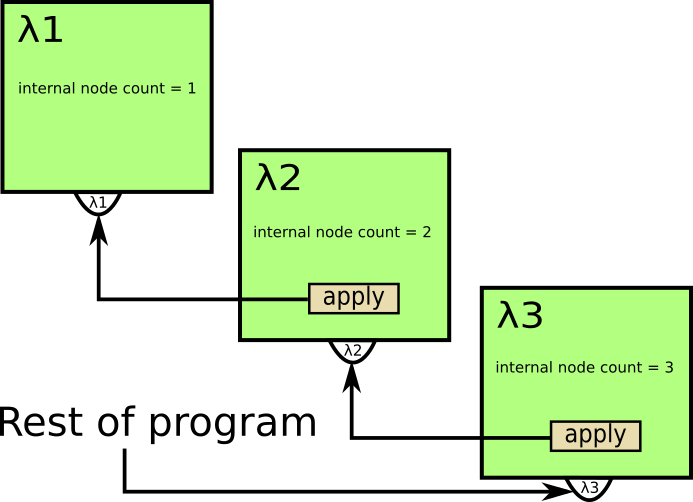
\includegraphics[width=0.75\textwidth]{figures/svg/inline_ordering_ex}
	\caption{An example of an RVSDG subgraph, depicting a function call
order in a program.}
	\label{fig:inline_ordering_ex}
\end{figure}

This example assumes the node count contained within each function created by
inlining to be the sum of the internal node counts of the original function and
the one inlined. In other words, no optimizations or other compiler techniques
are performed on the RVSDG during the traversal of the \applyNode s, or
before/after each inlining.

As our example shows, the order in which the \applyNode s are inlined matters.
And because the order matters, our inliner is able to traverse the \applyNode s
of the RVSDG given as input in either a \nolinebreak{top-down} order, or a \nolinebreak{bottom-up} order.
Section~\ref{sub:fw:call_site_visit_order} discusses ideas for potential work
for future research regarding the impact of the order of inlined call sites.

\subsection{Inlining a call site}
\label{sub:scheme:inlining_apply_nodes}

While there exist several~\cite{GHCPaper,AdaptvStratInlSubst} ways in which
inlining is performed, we decided upon our
approach~\cite{AdaptvCompilAndInlingWaterman} because it permits effective
testing for an apt heuristic when deciding on whether or not to inline a call
site.

As mentioned, all \applyNode s eligible for inlining get inlined based on the
same heuristic per run of our inliner. The heuristic is based on \textit{Inliner
Conditions} (ICs), such as the following:

\begin{itemize}
	\item \textit{Node Count} (NC)

The amount of nodes (operations) contained within the function invoked by the
\applyNode .

	\item \textit{Loop Nesting Depth} (LND)

The amount of nested loops the \applyNode~resides within.

	\item \textit{Static Call Count} (SCC)

The total amount of \applyNode s invoking the same function in the RVSDG given
as input.
\end{itemize}

These ICs and others described in Section~\ref{sub:meth:inlining_conditions}
allow us to write and \nolinebreak{re-write} the inlining heuristic effectively, by letting us
write them using \textit{Conjunctive Normal Form} (CNF). Thus, the CNFs written
for our inliner heuristic are written in the following fashion:
\lstinline"(NC < X || SCC < Y || (SCC < Z && LND > W))", where \lstinline!X!,
\lstinline!Y!, \lstinline!Z!, and \lstinline!W! are placeholder values.

While the work of Waterman~\cite{AdaptvCompilAndInlingWaterman}, which our
approach builds upon, utilizes a hillclimber algorithm to adaptively find decent
values for the placeholder variables for each individual run of the compiler,
this is outside the scope of our project.
